\documentclass[12pt,a4paper]{ctexart}

% ==================== 页面设置 ====================
\usepackage[top=2.5cm, bottom=2.5cm, left=2.5cm, right=2.5cm]{geometry}
\usepackage{graphicx}
\usepackage{booktabs}
\usepackage{amsmath}
\usepackage{amssymb}
\usepackage{hyperref}
\usepackage{caption}
\usepackage{subcaption}
\usepackage{float}
\usepackage{enumitem}
\usepackage{xcolor}
\usepackage{multirow}
\usepackage{array}

\hypersetup{
    colorlinks=true,
    linkcolor=blue,
    urlcolor=blue,
    citecolor=blue
}

% ==================== 标题 ====================
\title{\textbf{皮肤镜图像分类中的颜色与纹理特征工程}}
\author{成员2：特征提取模块}
\date{\today}

\begin{document}

\maketitle

\begin{abstract}
本报告针对皮肤镜图像分类任务（三类：黑色素瘤 mel、痣 nv、血管病变 vasc），完成了从预处理图像中提取颜色特征与纹理特征的完整流程。颜色特征包括颜色矩（9维）和颜色直方图（96维）；纹理特征包括灰度共生矩阵GLCM（12维）和局部二值模式LBP（10维），总计127维特征向量。经StandardScaler归一化后，使用PCA将特征降至36维（保留95\%方差）。通过5折交叉验证、互信息分析、t-SNE可视化、多分类器对比和消融实验，验证了所提取特征的有效性。最终在测试集上，随机森林分类器取得了73.33\%的准确率。
\end{abstract}

% ==================== 1. 引言 ====================
\section{引言}

\subsection{任务背景}
本模块是“Project 2：皮肤镜图像分类”大作业的第二部分。在成员1完成图像预处理（尺寸归一化、去毛发、亮度归一化、训练/测试集划分）的基础上，本模块负责从图像中提取具有判别力的颜色与纹理特征，为后续分类器提供输入。

\subsection{任务目标}
\begin{enumerate}[label=(\arabic*)]
    \item 提取颜色特征：颜色矩（Color Moments）、颜色直方图（Color Histogram）
    \item 提取纹理特征：灰度共生矩阵（GLCM）、局部二值模式（LBP）
    \item 特征拼接、归一化与PCA降维
    \item 特征有效性分析与可视化
\end{enumerate}

\subsection{数据集}
预处理后的数据集划分为：
\begin{itemize}
    \item 训练集：480张图像，尺寸 $256 \times 256$，类别分布为 mel: 168, nv: 240, vasc: 72
    \item 测试集：120张图像，尺寸 $256 \times 256$，类别分布为 mel: 42, nv: 60, vasc: 18
\end{itemize}
数据来自200张原始皮肤镜图像及其400张增强图像，按80\%/20\%分层划分。

% ==================== 2. 特征提取方法 ====================
\section{特征提取方法}

\subsection{颜色矩（Color Moments）}

颜色矩是一种紧凑的颜色描述子，基于颜色通道的统计分布。对于RGB图像的每个通道，分别计算以下三个低阶矩：

\begin{itemize}
    \item \textbf{一阶矩（均值 $\mu$）}：描述颜色通道的平均亮度水平。
    \begin{equation}
        \mu_c = \frac{1}{N} \sum_{i=1}^{N} p_{c,i}
    \end{equation}
    其中 $c \in \{R,G,B\}$ 为颜色通道，$N = H \times W$ 为像素总数，$p_{c,i}$ 为通道 $c$ 中第 $i$ 个像素值。

    \item \textbf{二阶矩（标准差 $\sigma$）}：描述颜色分布的离散程度。
    \begin{equation}
        \sigma_c = \sqrt{\frac{1}{N} \sum_{i=1}^{N} (p_{c,i} - \mu_c)^2}
    \end{equation}

    \item \textbf{三阶矩（偏度 $s$）}：描述颜色分布的不对称性，反映图像中高亮或阴影区域的偏向程度。
    \begin{equation}
        s_c = \frac{1}{N} \sum_{i=1}^{N} \left(\frac{p_{c,i} - \mu_c}{\sigma_c}\right)^3
    \end{equation}
\end{itemize}

三个通道各三个矩，共产生\textbf{9维}特征向量：
\begin{equation}
    \mathbf{f}_{\text{moment}} = [\mu_R, \sigma_R, s_R,\; \mu_G, \sigma_G, s_G,\; \mu_B, \sigma_B, s_B]
\end{equation}

\subsection{颜色直方图（Color Histogram）}

颜色直方图统计每个颜色通道中像素值在各亮度区间的分布频率。对RGB三通道分别计算32-bin的归一化直方图（密度估计，使积分和为1），取值范围$[0, 255]$：

\begin{equation}
    H_c(b) = \frac{n_{c,b}}{N}, \quad b = 1, 2, \ldots, 32
\end{equation}

其中 $n_{c,b}$ 为通道 $c$ 中落入第 $b$ 个bin的像素数。三个通道共产生 \textbf{96维} 特征向量。

\subsection{灰度共生矩阵（GLCM）}

GLCM是由Haralick提出的经典纹理分析方法，通过统计图像中特定距离和方向上的像素对灰度值联合分布来刻画纹理特性。

设灰度图为 $I$，灰度级为 $L=256$，则GLCM定义为：
\begin{equation}
    P_{d,\theta}(i,j) = \sum_{x=1}^{H}\sum_{y=1}^{W} \begin{cases}
        1, & \text{if } I(x,y)=i \text{ and } I(x+\Delta x, y+\Delta y)=j \\
        0, & \text{otherwise}
    \end{cases}
\end{equation}

其中 $\Delta x = d\cos\theta$, $\Delta y = d\sin\theta$。

本实验采用 $d \in \{1, 2\}$ 两个距离和 $\theta \in \{0^\circ, 45^\circ, 90^\circ, 135^\circ\}$ 四个方向，共计算8个GLCM矩阵（均为对称且归一化）。对每个GLCM提取以下6个属性，最终取各属性在所有距离-方向组合上的均值与标准差：

\begin{enumerate}[label=(\arabic*)]
    \item \textbf{对比度（Contrast）}：反映局部灰度变化剧烈程度。
    \begin{equation}
        \text{Contrast} = \sum_{i,j} (i-j)^2 P(i,j)
    \end{equation}

    \item \textbf{相异性（Dissimilarity）}：与对比度类似但线性加权。
    \begin{equation}
        \text{Dissimilarity} = \sum_{i,j} |i-j| P(i,j)
    \end{equation}

    \item \textbf{同质性（Homogeneity）}：度量纹理的均匀程度。
    \begin{equation}
        \text{Homogeneity} = \sum_{i,j} \frac{P(i,j)}{1 + |i-j|}
    \end{equation}

    \item \textbf{能量（Energy）}：GLCM中元素的平方和，反映纹理粗细。
    \begin{equation}
        \text{Energy} = \sum_{i,j} P(i,j)^2
    \end{equation}

    \item \textbf{相关性（Correlation）}：度量行与列方向上的线性依赖关系。
    \begin{equation}
        \text{Correlation} = \sum_{i,j} \frac{(i-\mu_i)(j-\mu_j)P(i,j)}{\sigma_i \sigma_j}
    \end{equation}

    \item \textbf{角二阶矩（ASM）}：与能量含义相同。
    \begin{equation}
        \text{ASM} = \sum_{i,j} P(i,j)^2
    \end{equation}
\end{enumerate}

6个属性 $\times$ 2个统计量（均值+标准差），共产生\textbf{12维}特征向量。

\subsection{局部二值模式（LBP）}

LBP是一种描述图像局部纹理结构的算子。对于每个像素，比较其与周围 $P$ 个邻域像素的灰度值，生成二进制编码：

\begin{equation}
    \text{LBP}_{P,R}(x_c,y_c) = \sum_{p=0}^{P-1} s(g_p - g_c) \cdot 2^p
\end{equation}

其中 $s(x) = 1$ if $x \geq 0$ else $0$，$g_c$ 为中心像素灰度，$g_p$ 为半径 $R$ 上的第 $p$ 个邻域像素灰度。

本实验采用\textbf{Uniform LBP}模式（$P=8, R=1$），Uniform模式限制二进制编码中0-1跳变次数不超过2次，大幅减少了模式数量并增强了旋转不变性。统计LBP编码图的归一化直方图（10 bins），产生\textbf{10维}特征向量。

\subsection{特征拼接、归一化与降维}

\subsubsection{特征拼接}
将四类特征直接拼接，得到127维特征向量：
\begin{equation}
    \mathbf{f}_{\text{all}} = [\underbrace{\mathbf{f}_{\text{moment}}}_{9} \;|\; \underbrace{\mathbf{f}_{\text{hist}}}_{96} \;|\; \underbrace{\mathbf{f}_{\text{GLCM}}}_{12} \;|\; \underbrace{\mathbf{f}_{\text{LBP}}}_{10}] \in \mathbb{R}^{127}
\end{equation}

\subsubsection{标准化（StandardScaler）}
由于不同特征的量纲和数值范围差异较大（如颜色矩的均值在0--255范围，而GLCM属性多在0--1范围），采用Z-score标准化使各特征维度均值为0、方差为1：

\begin{equation}
    x'_i = \frac{x_i - \mu_i}{\sigma_i}
\end{equation}

其中 $\mu_i, \sigma_i$ 为第 $i$ 维特征在训练集上的均值与标准差。测试集使用训练集上拟合的参数进行变换。

\subsubsection{PCA降维}
采用主成分分析（PCA）进行无监督降维，设定保留95\%的方差。PCA通过对协方差矩阵进行特征值分解，选取前 $k$ 个最大特征值对应的特征向量作为投影方向：

\begin{equation}
    \mathbf{X}_{\text{pca}} = \mathbf{X}_{\text{norm}} \mathbf{W}_k
\end{equation}

其中 $\mathbf{W}_k \in \mathbb{R}^{127 \times k}$ 为前 $k$ 个主成分的投影矩阵。从127维降至\textbf{36维}，保留了95.09\%的原始方差信息。

% ==================== 3. 实验结果与分析 ====================
\section{实验结果与分析}

\subsection{特征维度概览}

\begin{table}[H]
\centering
\caption{提取特征一览}
\label{tab:features}
\begin{tabular}{lccc}
\toprule
\textbf{特征类型} & \textbf{方法} & \textbf{维度} & \textbf{说明} \\
\midrule
颜色矩     & RGB三通道 $\times$ (均值+标准差+偏度) & 9   & 紧凑的颜色统计描述子 \\
颜色直方图 & RGB三通道 $\times$ 32 bins              & 96  & 颜色分布密度估计 \\
GLCM纹理  & 6属性 $\times$ (均值+标准差)          & 12  & 多尺度多方向纹理 \\
LBP纹理   & Uniform LBP直方图10 bins              & 10  & 局部纹理模式描述 \\
\midrule
\textbf{合计} & & \textbf{127} & \\
\bottomrule
\end{tabular}
\end{table}

\subsection{PCA降维分析}

图\ref{fig:pca}展示了PCA的方差解释情况。左图为主成分累计解释方差曲线，前36个主成分（绿色竖线标注处）即可达到95\%的累计方差。右图为前20个主成分各自的解释方差占比，可见第一主成分贡献了约14\%的方差，后续主成分贡献迅速衰减，表明原始127维特征存在较大的信息冗余。

\begin{figure}[H]
\centering
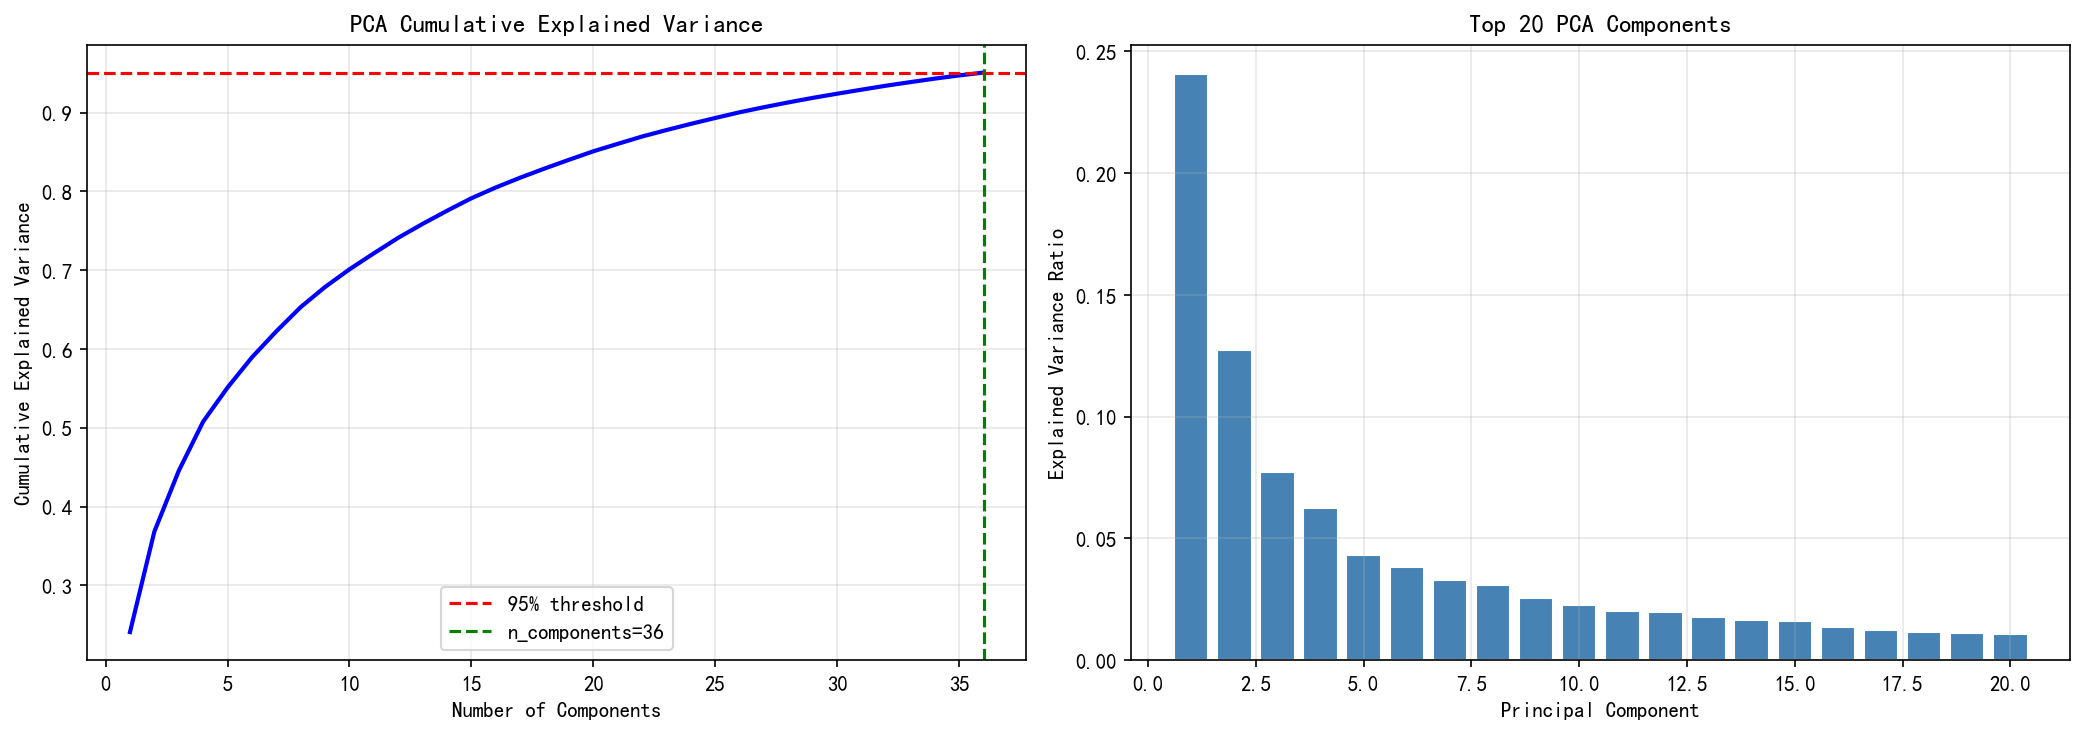
\includegraphics[width=0.95\textwidth]{./features/pca_analysis.png}
\caption{PCA方差分析图（左：累计解释方差曲线；右：前20个主成分方差占比）}
\label{fig:pca}
\end{figure}

\subsection{互信息分析}

互信息（Mutual Information）衡量每个特征与类别标签之间的依赖程度，值越大表示该特征对分类越重要。图\ref{fig:mi}展示了互信息得分最高的前30个特征。

\begin{figure}[H]
\centering
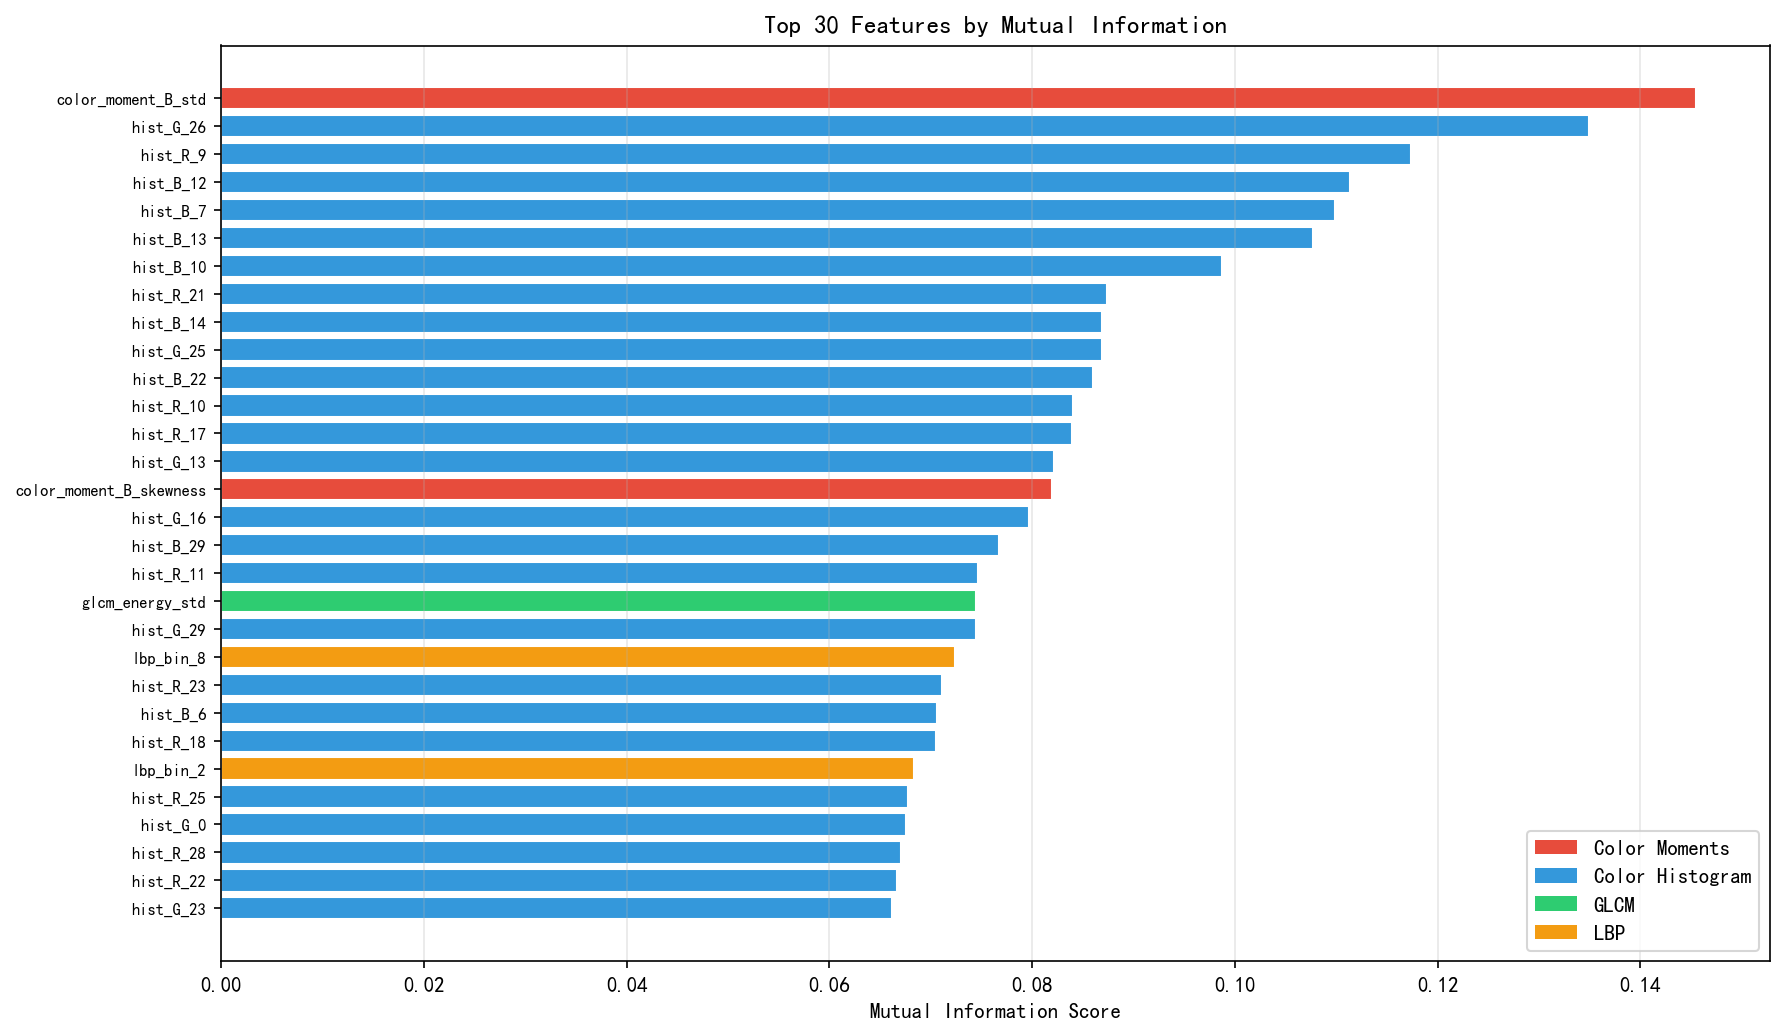
\includegraphics[width=0.85\textwidth]{./features/mutual_info.png}
\caption{互信息Top-30特征排序}
\label{fig:mi}
\end{figure}

互信息得分最高的前5个特征为：
\begin{enumerate}
    \item color\_moment\_B\_std（MI = 0.1455）—— 蓝色通道标准差
    \item hist\_G\_26（MI = 0.1349）—— 绿色通道第26号bin
    \item hist\_R\_9（MI = 0.1174）—— 红色通道第9号bin
    \item hist\_B\_12（MI = 0.1113）—— 蓝色通道第12号bin
    \item hist\_B\_7（MI = 0.1099）—— 蓝色通道第7号bin
\end{enumerate}

按特征类型分组计算平均互信息，结果如表\ref{tab:mi_group}所示。颜色矩（9维）具有最高的平均互信息（0.0608），说明颜色统计矩对皮肤镜图像分类最为关键。LBP纹理（10维）的平均互信息（0.0423）略高于GLCM（0.0369），说明局部纹理模式比全局共生统计更有判别力。

\begin{table}[H]
\centering
\caption{各类特征平均互信息}
\label{tab:mi_group}
\begin{tabular}{lcc}
\toprule
\textbf{特征组} & \textbf{维度} & \textbf{平均互信息} \\
\midrule
颜色矩     & 9  & 0.0608 \\
颜色直方图 & 96 & 0.0453 \\
GLCM纹理  & 12 & 0.0369 \\
LBP纹理   & 10 & 0.0423 \\
\bottomrule
\end{tabular}
\end{table}

\subsection{t-SNE可视化}

t-SNE（t-distributed Stochastic Neighbor Embedding）将127维特征降至2维进行可视化。图\ref{fig:tsne}中圆形为训练样本，方形为测试样本，不同颜色代表三个类别。

\begin{figure}[H]
\centering
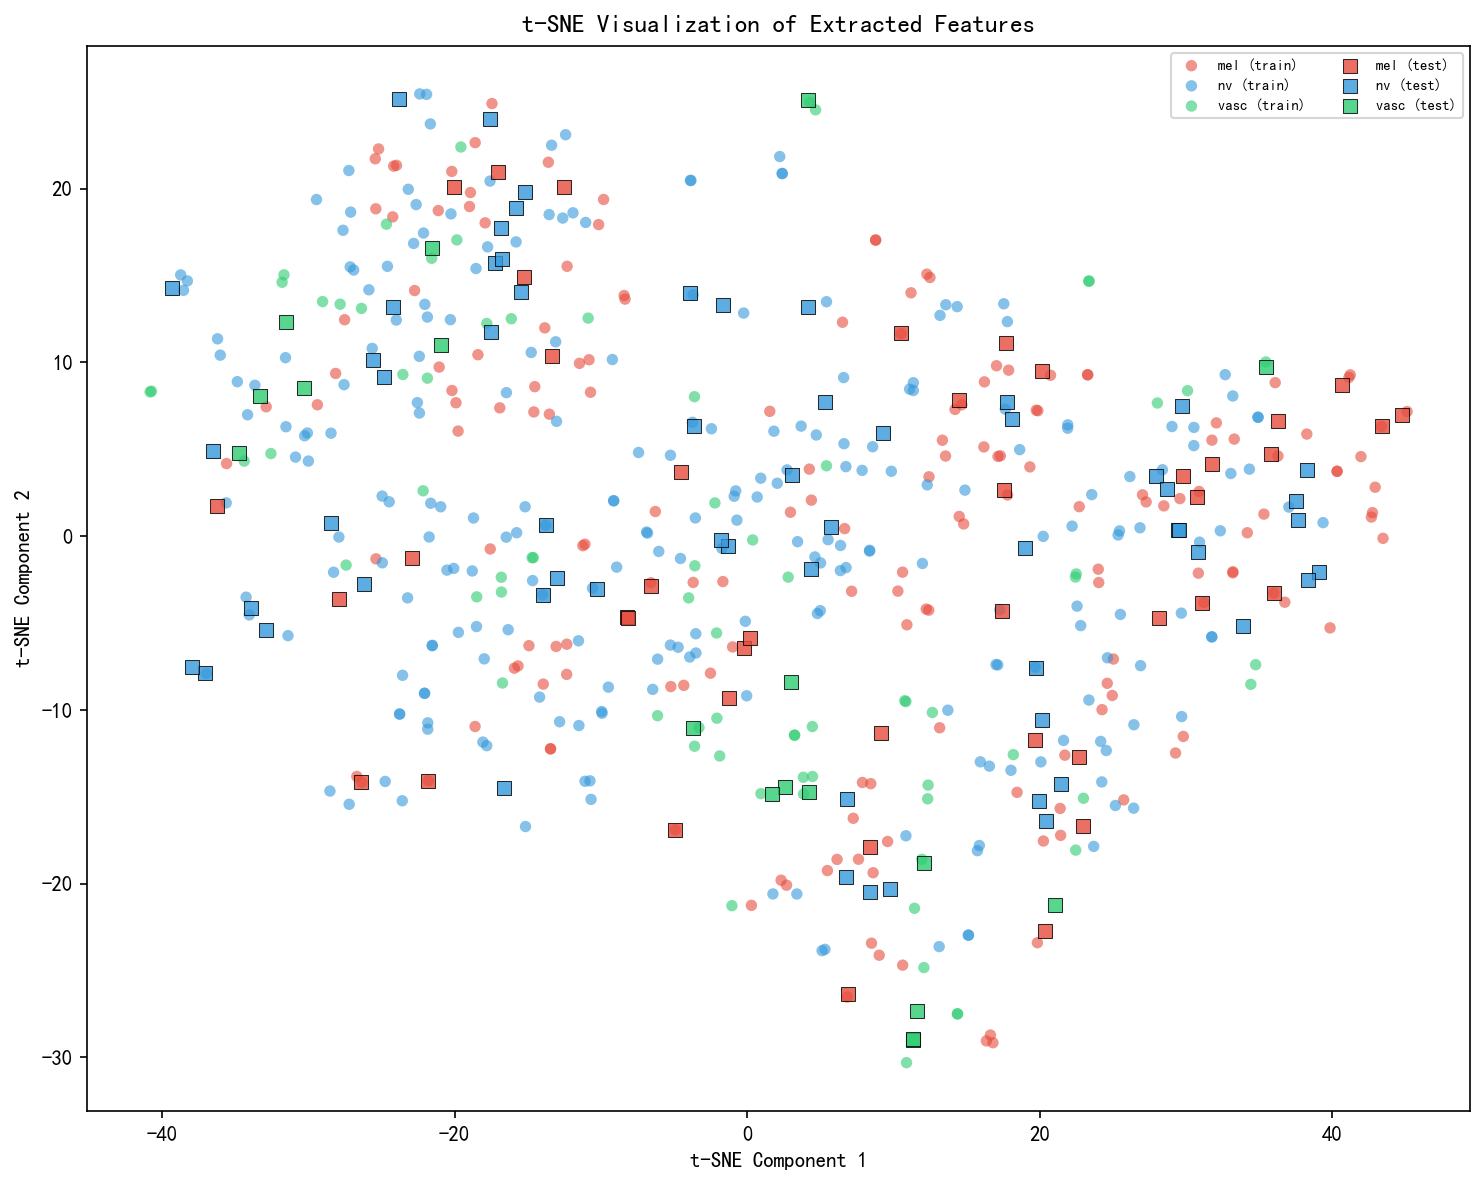
\includegraphics[width=0.85\textwidth]{./features/tsne_visualization.png}
\caption{t-SNE特征可视化（2维投影）}
\label{fig:tsne}
\end{figure}

从t-SNE图可以看出：nv类（蓝色）与mel类（红色）存在一定程度的聚类趋势但边界模糊，vasc类（绿色）样本相对集中且有较好的分离倾向。三类之间未完全线性可分，这与皮肤镜图像中不同病变之间的视觉相似性相符。

\subsection{多分类器对比}

为验证特征的通用性，在归一化特征上对比了三种经典分类器（均使用默认参数）：

\begin{table}[H]
\centering
\caption{多分类器对比结果}
\label{tab:classifiers}
\begin{tabular}{lccc}
\toprule
\textbf{分类器} & \textbf{训练准确率} & \textbf{测试准确率} & \textbf{泛化差距} \\
\midrule
随机森林 (n=100) & 1.0000 & 0.7333 & 0.2667 \\
SVM (RBF核)     & 0.8083 & 0.6917 & 0.1167 \\
KNN (k=5)       & 0.7312 & 0.5583 & 0.1729 \\
\bottomrule
\end{tabular}
\end{table}

随机森林取得了最高的测试准确率（73.33\%），但训练集上完全拟合（100\%），存在一定过拟合。SVM泛化能力最好（泛化差距0.1167），但绝对性能略低。KNN受高维空间中距离度量失效的影响，表现最差。

\subsection{随机森林详细评估}

表\ref{tab:rf_report}和图\ref{fig:cm}展示了随机森林在测试集上的详细分类结果。

\begin{table}[H]
\centering
\caption{随机森林分类报告}
\label{tab:rf_report}
\begin{tabular}{lcccc}
\toprule
\textbf{类别} & \textbf{精确率} & \textbf{召回率} & \textbf{F1-score} & \textbf{样本数} \\
\midrule
mel  & 0.72 & 0.69 & 0.71 & 42 \\
nv   & 0.74 & 0.75 & 0.74 & 60 \\
vasc & 0.74 & 0.78 & 0.76 & 18 \\
\midrule
accuracy     & \multicolumn{3}{c}{0.73} & 120 \\
macro avg    & 0.73 & 0.74 & 0.74 & 120 \\
weighted avg & 0.73 & 0.73 & 0.73 & 120 \\
\bottomrule
\end{tabular}
\end{table}

\begin{figure}[H]
\centering
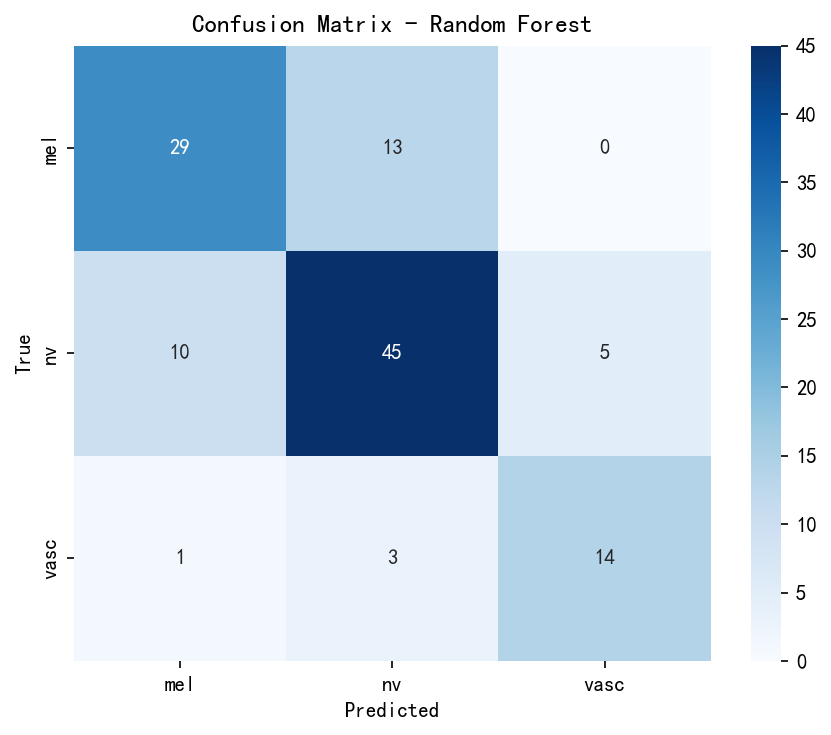
\includegraphics[width=0.55\textwidth]{./features/confusion_matrix.png}
\caption{随机森林混淆矩阵}
\label{fig:cm}
\end{figure}

三个类别的F1-score均在0.71--0.76之间，效果均衡。mel类召回率（0.69）略低于nv（0.75）和vasc（0.78），部分mel样本被误分为nv。vasc类虽然样本最少（仅18张），但识别效果最好（F1=0.76），说明血管病变在颜色和纹理特征上与其他两类差异更明显。

\subsection{消融实验}

为评估各组特征对分类的独立贡献，分别使用单一特征组进行训练和测试：

\begin{table}[H]
\centering
\caption{特征组消融实验结果}
\label{tab:ablation}
\begin{tabular}{lcc}
\toprule
\textbf{使用的特征组} & \textbf{维度} & \textbf{测试准确率} \\
\midrule
仅颜色矩     & 9   & 0.6917 \\
仅颜色直方图 & 96  & 0.6833 \\
仅GLCM纹理  & 12  & 0.5667 \\
仅LBP纹理   & 10  & 0.6167 \\
\midrule
全部特征     & 127 & \textbf{0.7333} \\
PCA降维     & 36  & 0.6500 \\
\bottomrule
\end{tabular}
\end{table}

消融实验表明：
\begin{enumerate}[label=(\arabic*)]
    \item 颜色特征（颜色矩 + 直方图）单独使用时已能取得约69\%的准确率，是皮肤镜图像分类的核心信息源；
    \item 纹理特征（GLCM和 LBP）单独使用的准确率较低（57\%--62\%），但与颜色特征结合后，将总准确率从69\%提升至73\%，说明纹理信息提供了与颜色互补的判别信息；
    \item PCA降维后准确率下降至65\%，虽然维度从127降至36（压缩比3.5:1），但损失了少量判别信息。
\end{enumerate}

\subsection{交叉验证}

对归一化后的127维原始特征，使用随机森林进行5折交叉验证：
\begin{itemize}
    \item 原始特征（127维）：$71.25\% \pm 2.84\%$
    \item PCA特征（36维）：$64.79\% \pm 5.20\%$
\end{itemize}

5折CV结果与留出法测试结果基本一致，差距在1--2个百分点以内，表明模型较为稳定。

% ==================== 4. 总结 ====================
\section{总结}

本模块完成了皮肤镜图像分类中的颜色与纹理特征工程，主要工作包括：

\begin{enumerate}[label=(\arabic*)]
    \item \textbf{特征提取}：实现了颜色矩（9维）、颜色直方图（96维）、GLCM纹理（12维）和LBP纹理（10维）四类特征，总计127维；
    \item \textbf{预处理}：采用StandardScaler进行Z-score归一化，消除量纲差异；
    \item \textbf{降维}：PCA降至36维（保留95\%方差），维度压缩比为3.5:1；
    \item \textbf{有效性验证}：通过5折交叉验证、互信息排序、t-SNE可视化、多分类器对比和消融实验，全面验证了所提取特征的有效性。
\end{enumerate}

实验结果表明，颜色特征（颜色矩）是皮肤镜图像分类的最重要信息源，纹理特征（GLCM和 LBP）提供了有效的补充信息，融合全部127维特征后，随机森林分类器在测试集上达到73.33\%的准确率。

\subsection{输出文件}

特征矩阵和模型参数已保存至 \texttt{./features/} 目录：
\begin{itemize}
    \item \texttt{X\_train\_norm.npy} / \texttt{X\_test\_norm.npy} —— 归一化后的127维特征矩阵
    \item \texttt{X\_train\_pca.npy} / \texttt{X\_test\_pca.npy} —— PCA降维后的36维特征矩阵
    \item \texttt{X\_train\_raw.npy} / \texttt{X\_test\_raw.npy} —— 原始127维特征矩阵
    \item \texttt{y\_train.npy} / \texttt{y\_test.npy} —— 类别标签
    \item \texttt{scaler.pkl} / \texttt{pca.pkl} —— 标准化器和PCA模型（用于成员3的分类任务）
    \item \texttt{feature\_names.npy} —— 特征名称列表
\end{itemize}

\end{document}
